\documentclass[a4paper,landscape,columns=3]{CheatSheet}
\usepackage{bbm}
\usepackage{listings}
\usepackage{tikz}
\usetikzlibrary{quantikz}

\title{Quantum Quick Reference}
\author{D. L. Yonge-Mallo}
\date{\today}
\begin{document}

% Abbreviations.
\newcommand{\pithalf}{\ensuremath{\frac{\pi t}{2}}}
\newcommand{\ipithalf}{\ensuremath{\frac{i\pi t}{2}}}
\newcommand{\one}{\ensuremath{\mathbbm{1}}}

\maketitle


\section{Basic definitions}

unitary
Hermitian


\section{Operators}




\section{Rotations}

% see 13269 for more notes

\begin{align*}
X^{t} &= \exp\left(\ipithalf\right)
\begin{bmatrix}
\cos\left(\pithalf\right) & -i\sin\left(\pithalf\right) \\
-i\sin\left(\pithalf\right) & \cos\left(\pithalf\right) \\
\end{bmatrix}\\
Y^{t} &= \exp\left(\ipithalf\right)
\begin{bmatrix}
\cos\left(\pithalf\right) & -\sin\left(\pithalf\right) \\
\sin\left(\pithalf\right) & \cos\left(\pithalf\right) \\
\end{bmatrix}\\
Z^{t} &= \exp\left(\ipithalf\right)
\begin{bmatrix}
\exp\left(-\ipithalf\right) & 0 \\
0 & \exp\left(\ipithalf\right) \\
\end{bmatrix}\\
\end{align*}

Recall that \(\exp(iAx) = \cos(x)\one + i\sin(A)X\).

% \section{Academic Research}

% \subsection{Game trees}

\section{Useful Circuit Identities}

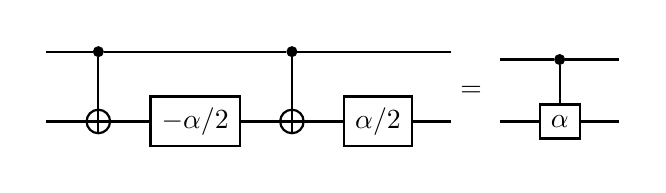
\begin{tikzpicture}
    \node[scale=1.0] {
        \begin{quantikz}
            & \ctrl{1} & \qw              & \ctrl{1} & \qw             & \qw \\
            & \targ{}  & \gate{-\alpha/2} & \targ{}  & \gate{\alpha/2} & \qw
        \end{quantikz}
        =
        \begin{quantikz}
            & \ctrl{1}      & \qw \\
            & \gate{\alpha} & \qw
        \end{quantikz}
    };
\end{tikzpicture}

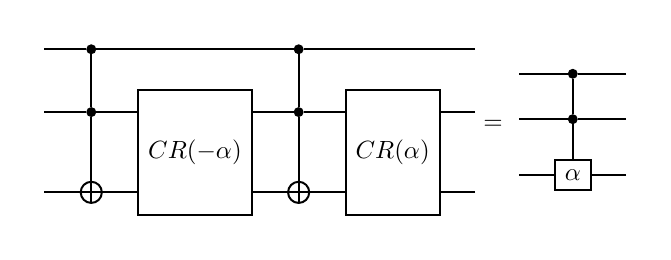
\begin{tikzpicture}
    \node[scale=0.9] {
        \begin{quantikz}
            & \ctrl{1} & \qw                   & \ctrl{1} & \qw                  & \qw \\
            & \ctrl{1} & \gate[2]{CR(-\alpha)} & \ctrl{1} & \gate[2]{CR(\alpha)} & \qw \\
            & \targ{}  & \qw                   & \targ{}  & \qw                  & \qw
        \end{quantikz}
        =
        \begin{quantikz}
            & \ctrl{1}      & \qw \\
            & \ctrl{1}      & \qw \\
            & \gate{\alpha} & \qw
        \end{quantikz}
    };
\end{tikzpicture}

\section{Fidelities}

% see 15318, 15368-9

\section{Variational Quantum Eigensolver (VQE)}

% see 15275

VQE: seek low-energy states of a quantum many-body system with a local Hamiltonian.

find eigenvalues of large matrix that represents Hamiltonian of a system
usually looking for ground state energy, but can also use to find additional eigenvalues for excited state energies

hybrid classical/quantum approach

can use to find min of any objective fn which can be expressed as quantum circuit

in variational methods, start with "best guess" or ansatz for ground state





\section{QAOA}

\section{Grover's search algorithm}
% see 15280

The Quantum Approximation Optimization Algorithm is...

% \section{Virtual Environments}
%
% For Cirq:
% \begin{lstlisting}
% mkvirtualenv cirq-py3 --python=/usr/bin/python3
% workon cirq-py3
% \end{lstlisting}
%
% For Qiskit:
% \begin{lstlisting}
% python3 -m venv QiskitDevenv
% source QiskitDevenv/bin/activate
% \end{lstlisting}

% \section{Installing packages from CTAN on macOS}
% 
% \begin{lstlisting}
% tlmgr install quantikz
% \end{lstlisting}


\end{document}
